\documentclass{article}

\usepackage{amssymb}
\usepackage{amsmath}
\usepackage[french]{babel}
\usepackage[utf8]{inputenc} 
\usepackage[T1]{fontenc}

\usepackage{graphicx}

\usepackage[a4paper,left=2cm,right=2cm,top=2cm,bottom=2cm]{geometry}

\usepackage{setspace}

\setlength{\parindent}{0cm}
\setlength{\parskip}{1ex plus 0.5ex minus 0.2ex}
\newcommand{\hsp}{\hspace{20pt}}
\newcommand{\HRule}{\rule{\linewidth}{0.5mm}}

\title{Compte rendu}
\author{Arthur Lacoin - Timothé Rios}

\date{}
    
\begin{document}

\begin{titlepage}
    \begin{sffamily}
    \begin{center}

        \textsc{\LARGE Lycée Lakanal}~\\[2cm]

        \HRule \\[0.4cm]
        { \huge \bfseries Simulation d'épidémies à l'aide d'automates cellulaires\\[0.4cm] }
    Un automate cellulaire est une matrice de cellules, chacune ayant un état, état appartenant à un ensemble prédéfini. L'état de chaque cellule peut varier au cours du temps suivant une fonction de transfert : l'état de la matrice à l'instant t+1 dépend ainsi de son état à l'instant t. L'automate doit donc posséder un état initial, c'est-à-dire la matrice des états initiaux des cellules.
        \HRule \\[2cm]
        \textsc{\Large Timothé Rios - Arthur Lacoin}\\[2cm]

    \end{center}
\end{sffamily}
\end{titlepage}

\tableofcontents

\begin{abstract}

Within the theme of transport, we have looked at how an epidemic spreads. To be able to represent this phenomenon, we chose to use a cellular automaton. A cellular automaton is a matrix of cells whose states vary over time. Here, at every moment, each cell can be Healthy, Sick, Deceased or Healed, according to its state as well as that of its neighbours at the moment before. Thus, with the information of an initial state, it is possible to materialize the spread of an epidemic. Of course, in order to accurately represent reality, it is necessary to make this model more complex by taking into account many factors that play a role in how a disease spreads.

\end{abstract}

\section{abstract}
	L'étude de la propagation des maladies est une science qui remonte à 1854, quand John Snow, un médecin britannique, étudia la propagation de l'épidémie de choléra dans les quartiers de Londres. Ce sont là les prémices de l'épidémiologie, étude du transport des infections. De nos jours les méthodes ont évolué, et on utilise principalement la méthode différentielle, que l'on présentera plus loin. Nous nous sommes attardés, ici, à la simulation par automate cellulaire.

\section{Première version}

\subsection{Présentation}

\subsubsection{Définition formelle}
	Un automate cellulaire est une matrice de cellules, chacune ayant un état, état appartenant à un ensemble prédéfini. L'état de chaque cellule peut varier au cours du temps suivant une fonction de transfert : l'état de la matrice à l'instant $t+1$ dépend ainsi de son état à l'instant $t$. L'automate doit donc posséder un état initial, c'est-à-dire la matrice des états initiaux des cellules.

\subsubsection{Historique}
	Les automates cellulaires sont plutôt récents. Ils ont été mis au point par John Von Neumann dans son étude des systèmes auto-réplicatifs dans les années 1940. Cette notion a été grandement popularisée par le "jeu de la vie" de John Conway, un automate cellulaire en 2 dimensions paru dans les années 1970. À ce jour, les automates cellulaires ont de nombreuses applications dans divers domaines :
	\begin{itemize}
	\item Diffusion d'un gaz en s'appuyant sur les équations de Navier-Stokes
	\item Simulation des feux de forêts
	\item Simulation du trafic routier
	\end{itemize}

\subsubsection{Notre automate cellulaire}
	Notre automate cellulaire est un automate en deux dimensions qui vise à simuler la propagation d'une épidémie. Les cellules ont donc un état parmi les 4 suivants : Sain, Malade, Guéri, Mort. Lorsqu'une cellule est saine, elle peut tomber malade avec une probabilité $p_1$ s'il y a des malades dans son entourage. Une cellule malade peut soit mourir avec une probabilité $p_2$ soit guérir avec une probabilité $p_3$. Les cellules mortes ou guéries restent dans cet état indéfiniment. La simulation s'arrête lorsqu'il n'y a plus de cellule malade.


\subsection{Résultats}

Lorsque l'on lance une simulation, on place l'épicentre de l'épidémie au centre de l'image, puis la maladie se déplace vers les bords de la grille pour finalement s'arrêter lorsqu'il n'y a plus d'infecté.

	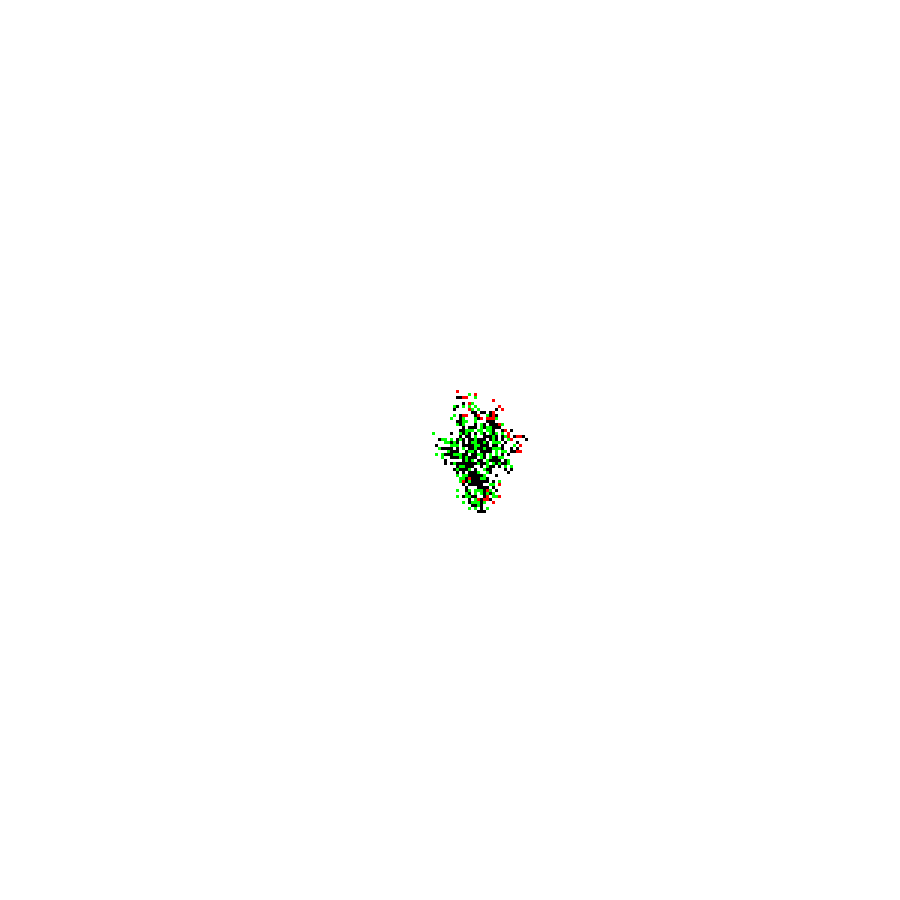
\includegraphics[scale=0.22]{Frame-36.png}
	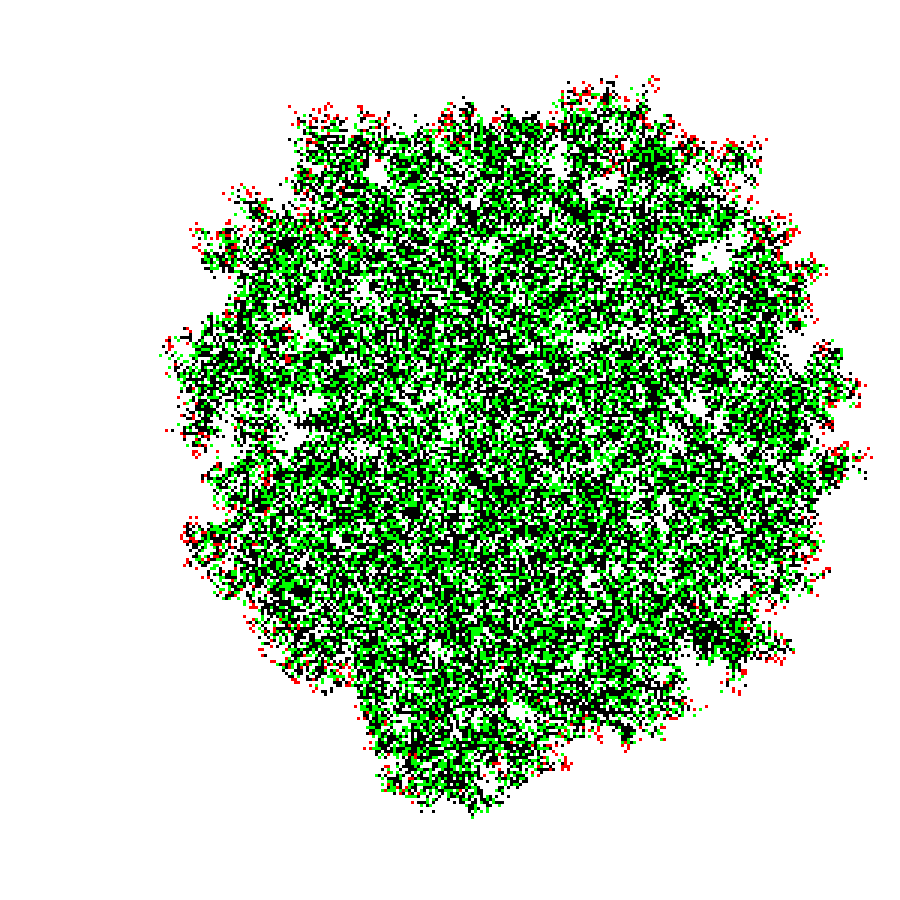
\includegraphics[scale=0.22]{Frame-195.png} 
	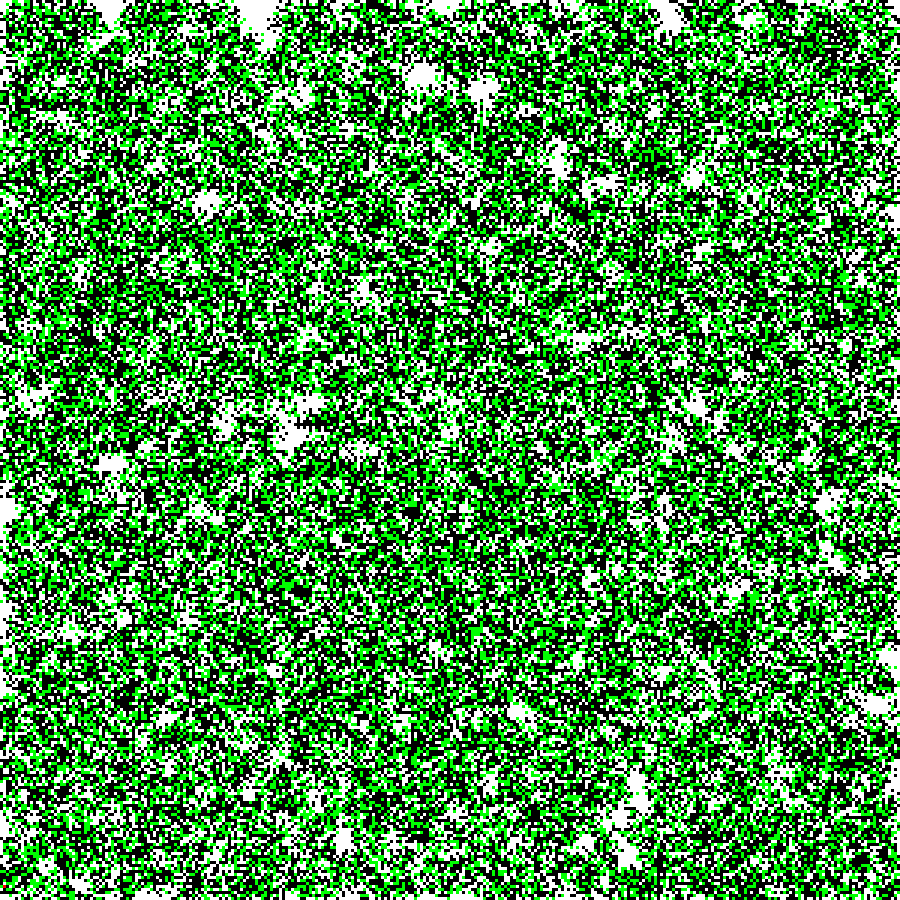
\includegraphics[scale=0.22]{Frame-412.png} 

	\begin{center}
	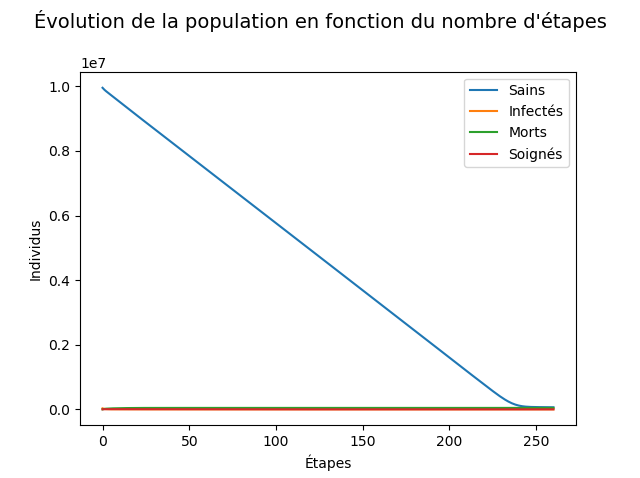
\includegraphics[scale=1.04]{Figure_1.png}
	Dans ce cas, $p_1 valait 0.2$, $p_2 valait 0.25$, $p_3 valait 0.2$, et la contamination possédait un rayon de 2 cellules.
	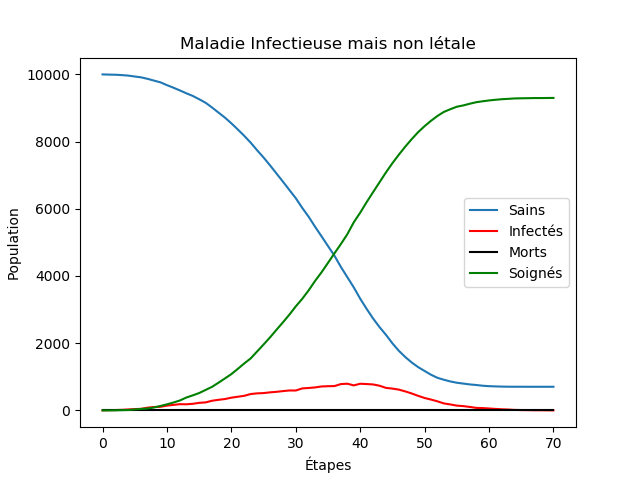
\includegraphics[scale=1.04]{Figure_2.png}
	Ici, nous pouvons voir l'exemple typique d'une maladie très infectieuse mais non létale, un rhume par exemple.
	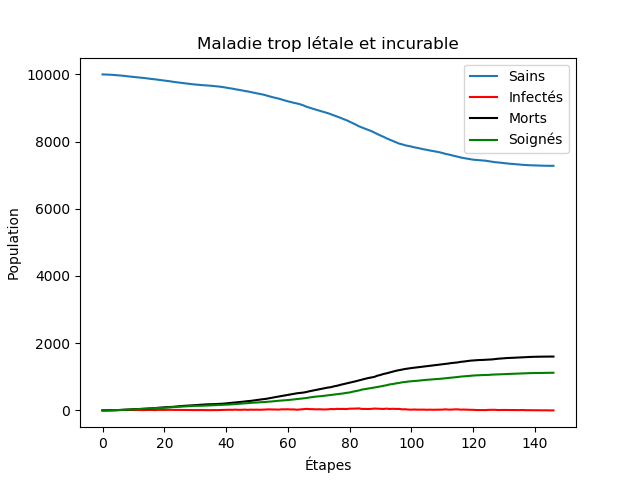
\includegraphics[scale=1.04]{Figure_3.png} 
Dans cet exemple, la maladie est trop létale pour pouvoir se propager efficacement : les infectés meurent sans avoir eu le temps de contaminer un de leurs voisins.

	\end{center}
\subsection{Limites}
	Cette version de l'automate cellulaire fournit déjà des résultats intéressants. Cependant, un grand nombre de paramètres a été négligé. Par exemple, il est ici supposé que la population est uniformément répartie, alors qu'en réalité cette densité dépend d'un nombre important de facteurs, comme le type de terrain, les constructions humaines (villes par exemple) ou les conditions météorologiques. De plus, nous supposons aussi que l'épidémie se déroule en un temps assez court pour que les décès naturels et les naissances soient négligeables, tout comme nous négligeons les mesures que pourraient prendre certains gouvernements en cas de pandémies majeures.
	
	
	
\section{Deuxième version}

\subsection{Présentation}
	Ce deuxième automate prend en compte plus de paramètres : 
	\begin{itemize}
	\item Nous avons cette fois considéré les cellules comme des zones géographiques plutôt que des individus, ayant une population ainsi qu'une répartition Sains-Malades-Morts-Guéris propre.
	\item Nous avons pris en compte les densités de population, celles-ci dépendant du 'type' de case, à savoir Ville, Campagne, Montagnes ou Route.
	\item Nous avons pris en compte les mouvements de population, en fonction de deux paramètres : La probabilité qu'une partie de population quitte une case, et la probabilité qu'une case a d'attirer la population des cases adjacentes.
	\end{itemize}
	
	Ces ajouts de paramètres permettent une simulation plus fine et plus proche de la réalité. Cela permet d'utiliser de bien meilleure façon les automates cellulaires, qui ont pour avantage de prendre en compte les paramètres géographiques de la simulation.


\subsection{Résultats}

Dans ce cas, nous n'avons pas pu afficher l'état complet d'une case sur une seule image, et il a fallu séparer en 4 les résultats. Voici les résultats avec les individus sains : \\[0.6cm]
%\includegraphics[scale=1.3]{2_sains.png} 
%\includegraphics[scale=1.3]{26_sains.png} 
%\includegraphics[scale=1.3]{64_sains.png} 


\subsection{Comparaison}

\nocite{*}
\bibliographystyle{plain}
\bibliography{bibliographie}

\end{document}